\documentclass[letterpaper,11pt]{article}

\usepackage{graphicx}
\usepackage{multicol}
\usepackage{fullpage}
\usepackage{csquotes}
\usepackage[margin=0.75in,letterpaper]{geometry}
\setlength{\footskip}{15pt}
\setlength{\belowcaptionskip}{9pt}
\usepackage{floatflt}
\usepackage{xspace}
\usepackage[margin=1cm,skip=9pt]{caption}
\usepackage{censor}
\usepackage{ulem}
\linespread{0.95}
\def\degC{$^{\circ}$C }
\def\degf{$^{\circ}$F }
\def\vol #1 {{\bf #1}, $\;\;$}
\def\refer{\par\noindent\hangindent\parindent\hangafter1}


\title{\vspace{-2.0cm}Herzmann Family Redacted Christmas Letter 2019}
\author{Daryl Herzmann${}^1$, Elizabeth Herzmann${}^2$, Margaret 
Herzmann${}^3$,\\
Robert Herzmann${}^4$, AND Charlotte Herzmann${}^5$ \\
\it{${}^1$ Corresponding Author},
\it{${}^2$ Responsible Adult},
\it{${}^3$ Senior Child},
\it{${}^4$ Growing Boy},
\it{${}^5$ Terrible Two}}
\date{21 December 2019}

\makeatletter
\newenvironment{tablehere}
  {\def\@captype{table}}
  {}

\newenvironment{figurehere}
  {\def\@captype{figure}}
  {}
\makeatother

\newcommand{\Line}[0]{%
  \rule{0cm}{0cm}\\\hrule\rule{0cm}{0cm}%
}

%\addtolength{\textheight}{1.5in}

\begin{document}
\maketitle
\vspace{-0.75cm}
\begin{abstract}
Attrition prevailed once again this year, so welcome back to another 
high production value installment
of our annual letter.  Last year's tome (Herzmann et al., 2018) was not properly
vetted and may have publicly released classified sources and methods.
Additionally, Daryl's mother's side of the family contains many Muellers 
and so we are likely related to \textit{Special Counsel Robert S. Mueller, III}.  
As such, this year's letter has been properly redacted before release pending
future court action.
\end{abstract}

\vspace{-0.5cm}
\Line
%\vspace{-0.5cm}

\begin{multicols}{2}

    
\section{Introduction} 

The size of our family was not modified this year and comprises Daryl
\enquote{Daryl} (41), Elizabeth \enquote{Liz} \censor{..},
Margaret \enquote{Maggie Moo} (6), Robert \enquote{Ro-Ro} (5), Charlotte
 \enquote{Charly Burger} (2), and one cat with a dog's name of Snoopy (11). 
The family implementation plan calls for size stability going forward.  All
family members managed to stay out of jail this year, except \censor{.....}
who \blackout{disturbed the peace after watching} 
\textit{The Price is Right}. 

   
\subsection{Housing}

Our house, circa 1996 with an octagon window, remains located in the same
swank Ankeny, IA location.  The children have yet to destroy it. Our living
room painting of ducks flying needed moved to make space for more monthly
picture documentation of our children's development (Fig 1).  It remains to
be seen how far into the children's teenage years this will be permitted
to continue.

\bigskip

\begin{figurehere}
    \centering   
    \resizebox{.95\columnwidth}{!}{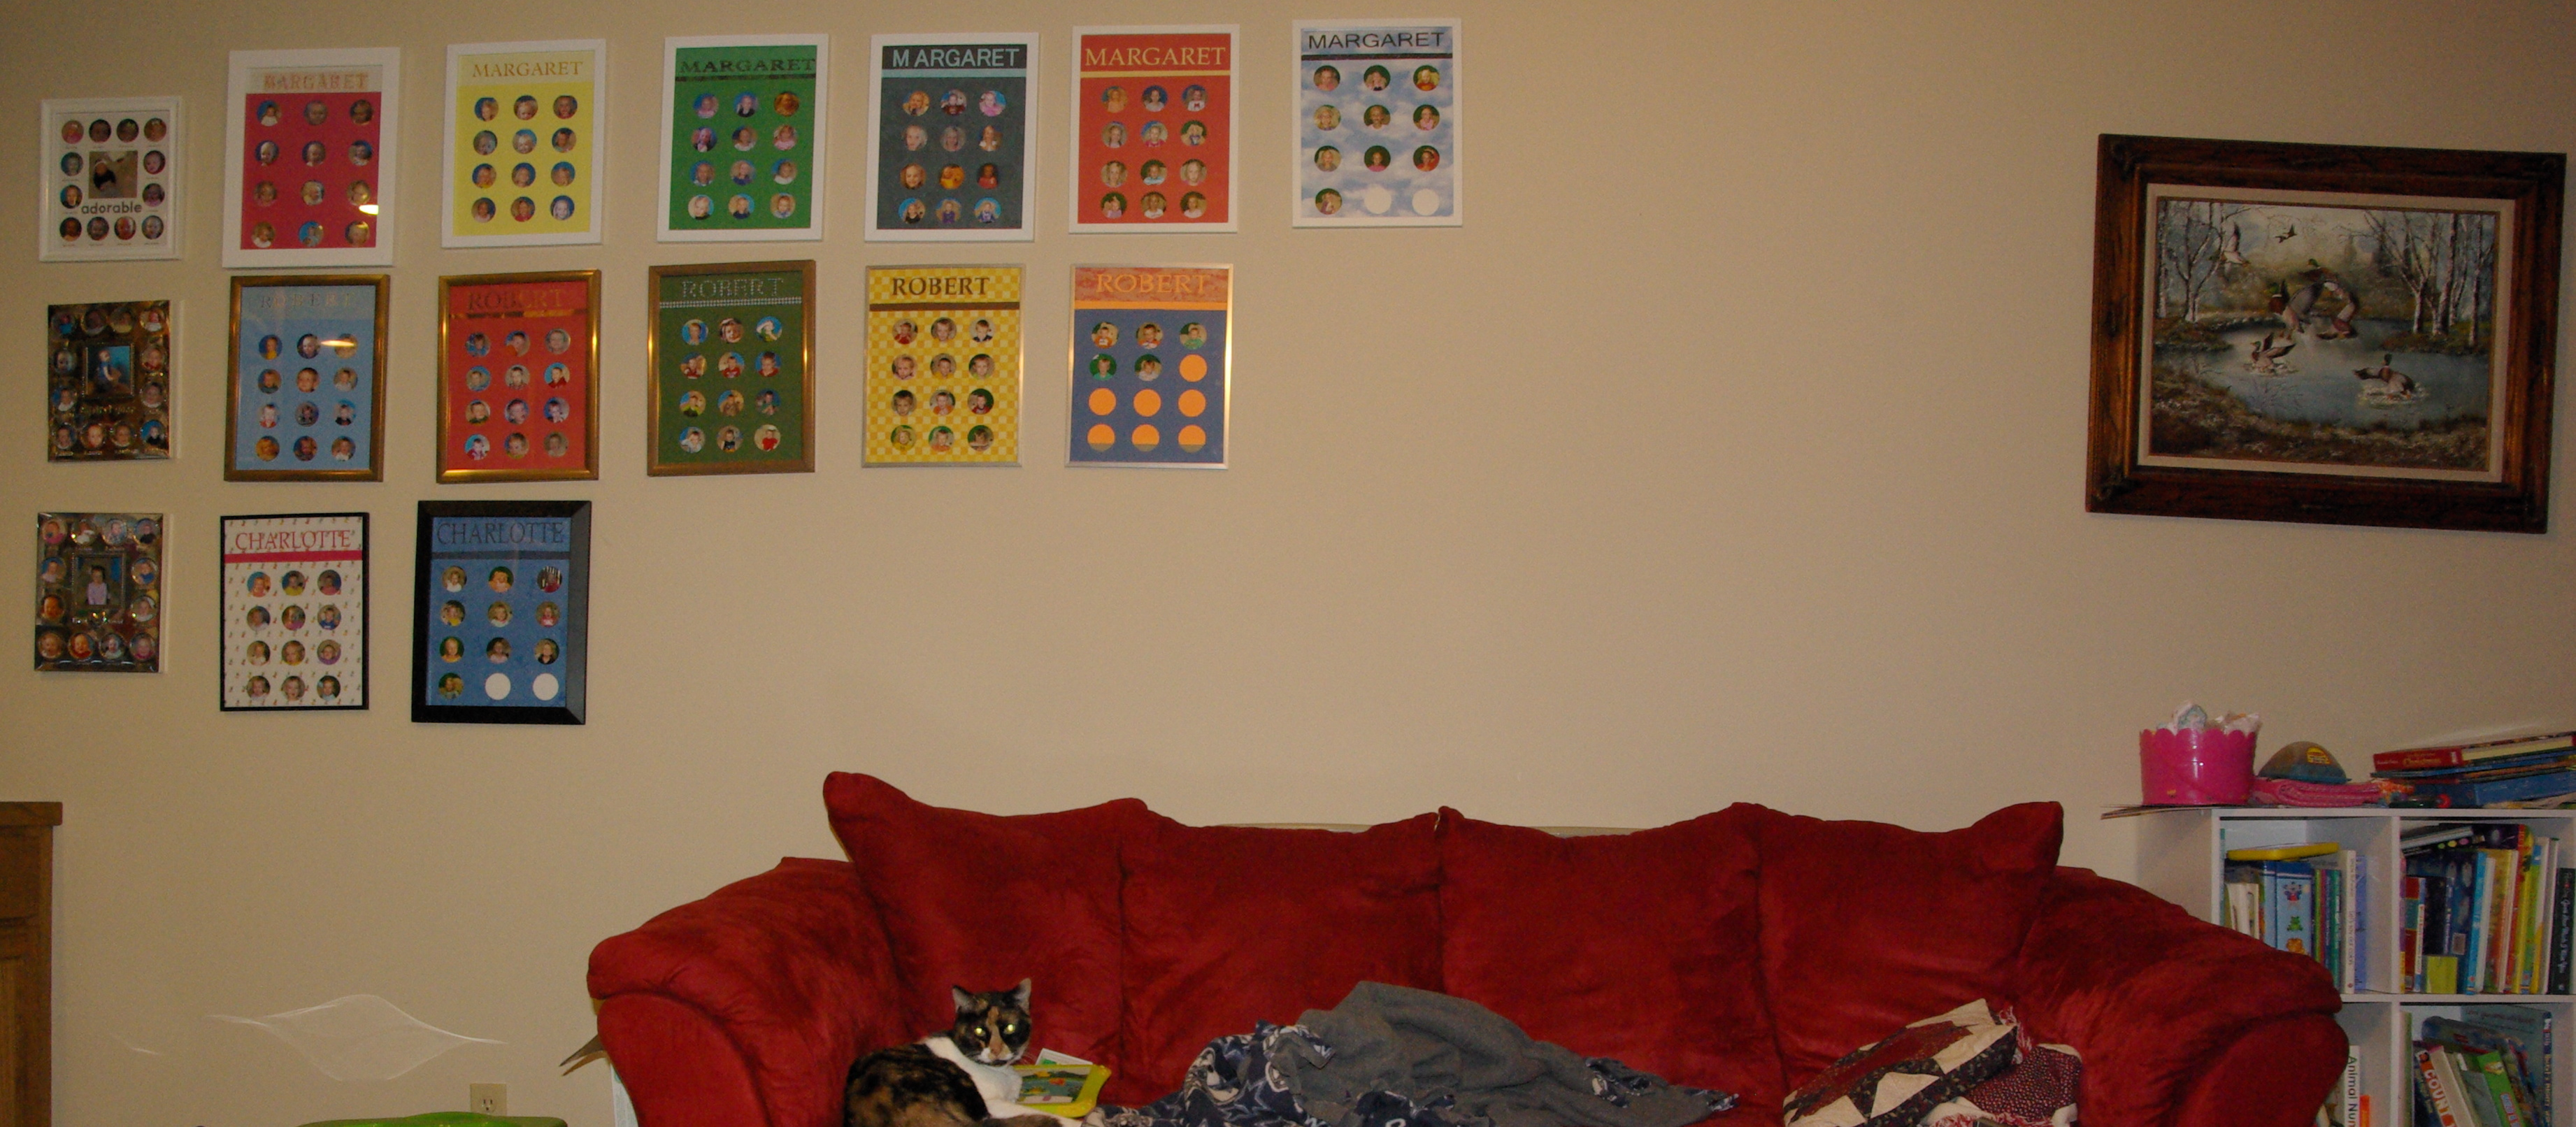
\includegraphics[angle=0]{plots/livingroom.eps}}
    \caption{Pedantic accounting of monthly development overseen by Snoopy the cat.}
   \end{figurehere}


\subsection{Employment}

Daryl continues to trek each day to Ames to work at Iowa State University as
he doesn't know any better.  He mostly writes software bugs 
related to soil erosion modeling, agronomic databasing, and weather data
collection.  He also monitor's the government's \sout{weather} modification program
named \censor{HAARP}, which spreads \blackout{blah and blah} from commercial
airplanes.

Liz continues to indoctrinate 8th grade youth at Southview Middle School
here in Ankeny.  This is her second year at the school.  She trained hard this
year to run the Des Moines half marathon successfully in October.  Her finishing
time was \censor{2.75} hours. She is blessed
being a Catholic Catechist for high school youth at the church and teaching our
children about God.

The children all seek opportunistic and transient employment to collect whatever
free change they suspect a nearby adult may have to offer.  Once the transaction
completes, they demand transportation to nearby store to spend it on items such
as \textit{Lunchables}, \textit{Legos\texttrademark}, and/or toys.  They all
still believe that shiny pennies have meaningful value.

\section{Miss Charlotte}

Miss Charlotte's past year has lived up to the hype known as "Terrible Twos". She
has shown some interest in potty training, but is not there yet.  She insists that
momma be present for every activity.  She is a good child though and her language
skills are really good.  She is just a handful to deal with each day.

She enjoys fighting over toys and wrestling with her daddy. She wakes up extra
early each morning to ensure mommy and daddy are not subjected to the alarm clock.
She still likes pancakes, bacon, and yogurt.  For extra clarity and even after
affirmation, she repeats all statements many times to ensure listener understanding
and retention.

\section{Mr Robert}

Since he is a June baby, we had a choice of waiting a year to send Mr Robert to
Kindergarten this fall.  We decided to give it a shot and he greatly exceeded
our expectations.  He is very proud of the reading and writing progress he is
making and likes to earn rewards for his good behaviour at school.  His classroom
is right next to Miss Maggie and they look out for each other.  He even has the
same teacher that Miss Maggie had.

Mr Robert loves his Legos\texttrademark and bouncing various balls around the house with 
increasing levels of force.  He has not shown too much interest in sports yet,
but enjoys the finer things of life (Fig 2).  He does like watching football on TV and
cheers for whichever team has an animal for a mascot.

\bigskip

\begin{figurehere}
 \centering   
 \resizebox{.95\columnwidth}{!}{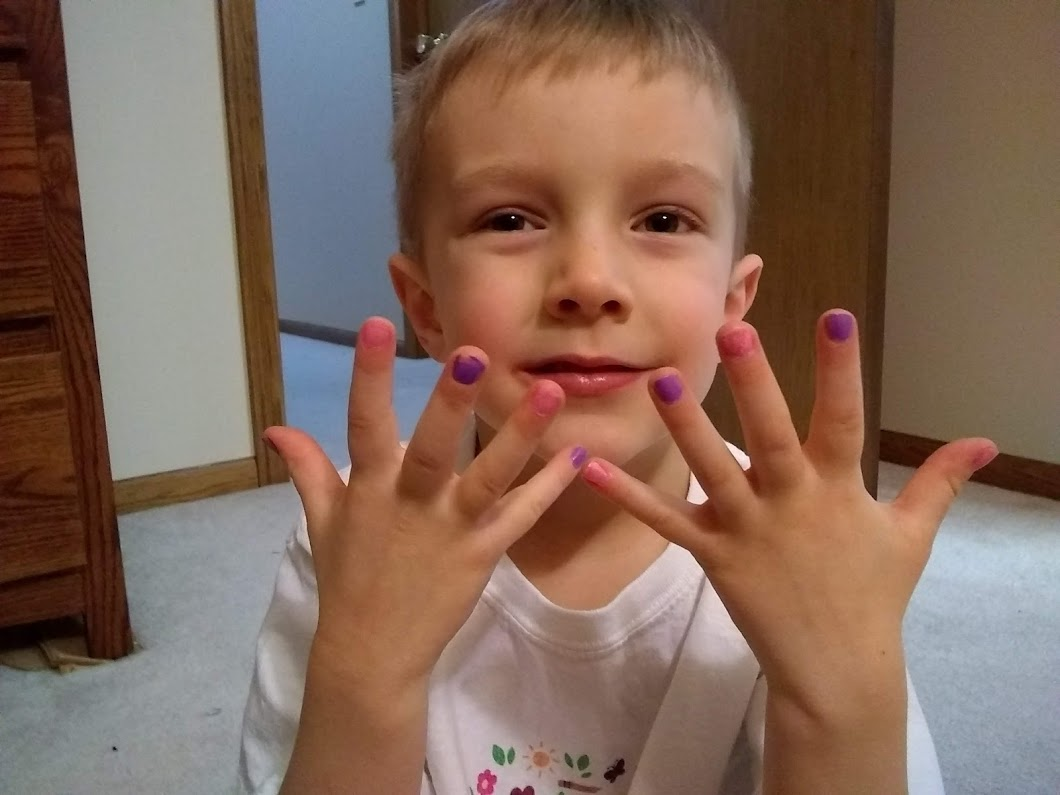
\includegraphics[angle=0]{plots/f3_2019.eps}}
 \caption{Future embarrassing picture of Mr Robert enjoying getting his finger nails painted.}
\end{figurehere}

\bigskip

\section{Miss Maggie}

Miss Maggie is now a flourishing First Grader. In her spare time, she loves her
tap and ballet dance class.  She recently had a recital of the \enquote{Nutcracker}
and is now preparing for a spring season recital.  She also likes swimming,
bossing the younger children around, and she \censor{loves} her daddy very
much.  Her current reading list includes:
\enquote{Rainbow Magic}, \enquote{WellieWishers\texttrademark}, and
Christmas Stories.  Her birthday is coming up in January and has told her
friends to bring food donations, in leiu of gifts, for the food pantry (read: proud parents).

She does an excellent job looking out for Mr Robert at school and is very kind
to others she meets.  When asked what she would like you to know from her
section of this letter, she said to have a Merry Chirstmas.

\section{Summary}

Progress continues to be made and we are generally cash flow \censor{positive} at this
time, so we will continue to learn, love, and laugh together.  Liz and Daryl continue
to try to take things slowly and enjoy this precious time we have with the young
children (Fig 3).

\bigskip

\begin{figurehere}
 \centering   
 \resizebox{.95\columnwidth}{!}{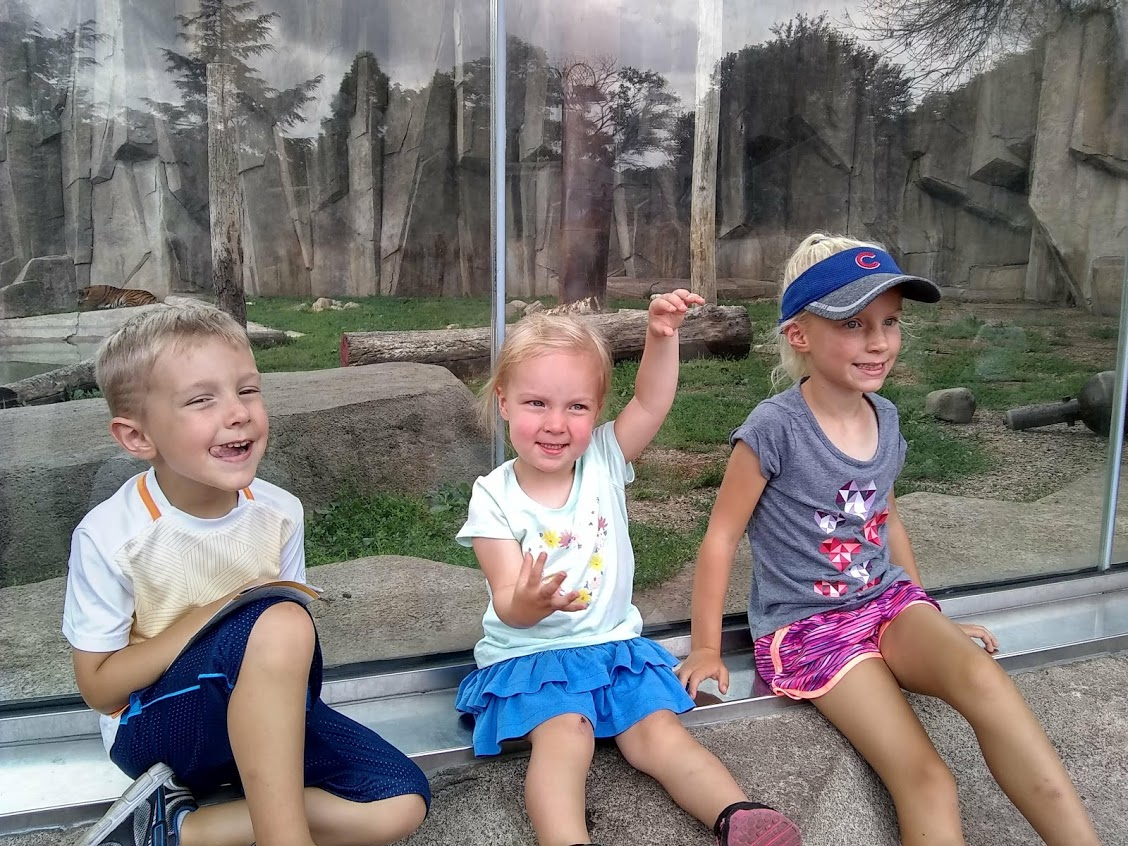
\includegraphics[angle=0]{plots/f2_2019.eps}}
 \caption{Children showing great faith that glass window will protect them from Milwaukee Zoo Tiger.}
\end{figurehere}

\bigskip

\emph{Acknowledgments} Our family wishes to thank you for the generous 
support, prayers, cards, gifts, and visits you have provided us in the past
year. With your continued support, this letter will be produced again
next year. Please note that the format chosen for this
correspondence was completely Daryl's idea and execution. Liz had marginal
editorial control. Full \LaTeX\xspace source can be found on Daryl's Github
page.

\section{References}

\refer Github, 2019: https://github.com/akrherz/me , visited 15 Dec 2019.
\refer Herzmann, Daryl E., et al. Herzmann Family Christmas Letter 2018.

\end{multicols}

\end{document}
